%%%% PLEASE REPLACE ENTIRELY WITH YOUR OWN CONTENT %%%%

\chapter[Estat de l'art]{Estat de l'art}
  
  \section{Internet of Medical Things (IoMT)} 
  L’Internet of Medical Things (IoMT) és una branca específica de l’Internet de les Coses (IoT) aplicada a l’àmbit sanitari. Consisteix en una xarxa creixent de dispositius mèdics intel·ligents que poden recopilar, processar i transmetre dades clíniques amb l’objectiu de millorar la qualitat assistencial, facilitar el monitoratge de pacients i optimitzar els processos hospitalaris.

  Aquest ecosistema connectat inclou una gran varietat de dispositius, que poden ser tant portables com fixes, i que cobreixen des del seguiment de signes vitals fins al control automatitzat de tractaments. Alguns exemples habituals són:

  \begin{itemize}
    \item \textbf{Monitors cardíacs:} permeten controlar l’activitat del cor de manera contínua.
    \item \textbf{Pulsòmetres i termòmetres intel·ligents:} ofereixen dades precises i fàcilment accessibles.
    \item \textbf{Inhaladors i bombes d’insulina intel·ligents:} poden registrar l’ús i ajudar a ajustar el tractament.
    \item \textbf{Implants mèdics connectats: } permeten registar l'estat d'un pacient a temps complert. Per exemple marcapassos o neuroestimuladors.
    \item \textbf{Sistemes de dosificació automàtica de medicació:} especialment útils en pacients amb malalties cròniques.
    \item \textbf{Equips hospitalaris intel·ligents:} com llits monitoritzats o sistemes de seguiment de pacients dins d’unitats de cures intensives.
  \end{itemize}

  El creixement de l’IoMT s’ha vist impulsat per diversos factors, com la miniaturització dels sensors, el progrés tecnològic en dispositius mèdics, l’augment de la digitalització sanitària, i la necessitat creixent de models d’atenció centrats en el pacient i orientats a la prevenció i el seguiment continuat. A més, la pandèmia de la COVID-19 va accelerar l’adopció de solucions de monitoratge remot, que han consolidat l’ús d’aquest tipus de dispositius fora dels entorns hospitalaris convencionals.

  L’ús generalitzat d’aquesta tecnologia permet una atenció més personalitzada i basada en dades, alhora que facilita la detecció precoç de complicacions i una millor gestió dels recursos sanitaris. També contribueix a reduir la necessitat de desplaçaments i hospitalitzacions, millorant l’accessibilitat a l’atenció mèdica, especialment en zones rurals o amb menys infraestructures.
  
  Amb una adopció creixent tant en entorns clínics com domèstics, s’espera que l’IoMT sigui una peça clau en la transformació digital del sistema sanitari en els pròxims anys, aportant beneficis tant per als pacients com per als professionals de la salut. \cite{IoMTexp}

  \section{Seguretat en entorns IoMT}

  Donat el creixement de l'us de dispositius IoMT, aquesta mateixa expansió comporta un augment significatiu de la superfície d’exposició a ciberatacs. A més a més, s’espera que a mesura que avança la seva adopció, aquests dispositius siguin més determinants en les tasques mèdiques, la qual cosa pot impilcar una major criticitat en cas de ciberatac.

  A diferència dels sistemes informàtics convencionals, els dispositius IoMT sovint operen en entorns amb recursos computacionals limitats (processador, memòria, energia), i moltes vegades han estat dissenyats amb una orientació funcional, no pas de seguretat. Això els fa especialment vulnerables a atacants que poden es poden aprofitar de configuracions per defecte, manca d’actualitzacions, credencials febles o vulnerabilitats en els protocols de comunicació. A més, la connexió d’aquests dispositius mitjançant xarxes Wi-Fi o altres canals sense fils exposa el sistema a atacs com l’escolta (sniffing), suplantació de dispositius (spoofing), atacs de denegació de servei (DoS) entre altres.
  
  Un dels aspectes més crítics del risc en entorns IoMT és la naturalesa de les dades que gestionen. Les dades mèdiques són altament sensibles i personals. Un accés no autoritzat pot vulnerar drets fonamentals com la privacitat i tenir conseqüències legals greus per a les institucions sanitàries. En aquest context, la ciberseguretat en l’àmbit IoMT no es pot considerar un afegit posterior al desplegament dels sistemes, sinó un requisit fonamental des de la fase de disseny. Això, és especialment rellevant en entorns on les conseqüències d’un atac poden tenir un impacte directe sobre la salut i la seguretat física dels pacients.

  Però, és important destacar que la protecció dels sistemes IoMT també ha de ser escalable i adaptable. L’amenaça no és estàtica, i els vectors d’atac evolucionen constantment.
 
  Davant d’aquesta realitat, la recerca en ciberseguretat per a l’IoMT s’està orientant cada cop més cap a solucions dinàmiques, com ara IDS/IRS basats en aprenentatge automàtic que permetin detectar patrons anòmals de comportament i actuar de forma proactiva. En aquest sentit, la generació de datasets reals que simulin tant trànsit legítim com maliciós en entorns IoMT esdevé una peça clau per entrenar i validar aquestes solucions emergents. Aquestes solucions han estat tractades en artícles com \cite{iotthreadsexp}. També la caracterització de vulnerabilitats connegudes ha estat tractada en artícles com \cite{ciciomtexp} o \cite{lowrateDDoSexp} que han estat utlitzats com a referència per a la recopliació d'atacs i la generació de datasets.
  
  \section{Message Queuing Telemetry Transport (MQTT)}
  \label{sec:MQTT}
  El Message Queuing Telemetry Transport (MQTT) és un protocol de missatgeria lleuger dissenyat per a la comunicació entre dispositius amb recursos limitats en xarxes poc fiables o amb amplada de banda reduïda. Aquest protocol s’ha convertit en un estàndard de facto en moltes aplicacions IoT, inclòs l’àmbit de l’Internet of Medical Things (IoMT), per la seva eficàcia, simplicitat i facilitat de desplegament.
  
  Desenvolupat originalment per IBM l’any 1999, MQTT segueix un model de comunicació publish/subscribe, que afavoreix la desconnexió temporal dels nodes i la minimització de l’ús de la xarxa, dos requisits habituals en xarxes IoT. 
  
  En una arquitectura MQTT, el component central és el broker, un servidor que actua com a intermediari entre els dispositius que publiquen dades (publishers) i els que les reben (subscribers). Els dispositius no es comuniquen directament entre ells, sinó que ho fan a través del broker, que rep els missatges publicats en un tema determinat (tòpic) i els redirigeix als clients que s’han subscrit a aquest tema. Aquesta arquitectura desacoblada simplifica el disseny de sistemes escalables i resilients. A l’àmbit IoMT, aquesta estructura és especialment útil per gestionar sensors mèdics que generen dades de manera periòdica, com ara nivells de glucosa, senyals d’electrocardiograma (ECG), o mesures de tensió arterial. Aquests sensors poden publicar lectures de manera eficient al broker MQTT, i altres components del sistema (com bases de dades, aplicacions clíniques o sistemes d’alerta) poden consumir aquesta informació segons les seves necessitats. 
  
  El protocol MQTT opera habitualment sobre TCP/IP, utilitzant el port 1883 per a connexions no segures i el port 8883 quan es fa servir TLS (Transport Layer Security) per protegir la transmissió. Entre les característiques tècniques més destacades d’MQTT, podem ressaltar: 
  
  \begin{itemize}
      \item \textbf{Qualitat del servei (QoS):} MQTT ofereix tres nivells de abilitat en el lliurament de missatges, cosa que permet ajustar el comportament segons els requisits de l’aplicació. 
      \item \textbf{Sessions persistents:} Un missatge es pot marcar com a retained perquè quedi emmagatzemat al broker i sigui enviat automàticament als nous subscriptors del topic. Això permet garantir que les dades més recents estiguin disponibles en tot moment, encara que el dispositiu que les va enviar originalment ja no estigui actiu. 
      \item \textbf{Protocol lleuger:} Amb una capçalera mínima de només 2 bytes, MQTT genera molt poca sobrecàrrega, cosa que el fa extremadament ecient per dispositius amb CPU limitada, poca memòria RAM o connexions de xarxa inestables o intermitents.
      \item \textbf{Model desacoblat (publish/subscribe):} Els clients no necessiten conèixer ni l’adreça ni l’estat dels altres dispositius. Això facilita l’escalabilitat i la fexibilitat del sistema, ja que els rols de publicador i subscriptor poden canviar dinàmicament. 
      \item \textbf{Jerarquia de temes (topics):} Els topics MQTT segueixen una estructura jeràrquica cosa que permet l’ús de comodins ("+","\#"), fet que proporciona una gran fexibilitat, però també pot ser explotat maliciosament si no es controla adequadament. 
  \end{itemize}

Malgrat aquests avantatges, el protocol MQTT no està pensat amb la seguretat com a objectiu principal, cosa que el fa vulnerable en entorns crítics com l’IoMT si no s’hi afegeixen mecanismes de protecció. Les principals limitacions de seguretat inclouen:  
  \begin{itemize} 
      \item \textbf{El broker com a punt crític:} El broker MQTT és un únic punt de fallada. Si és compromès o queda saturat, tota la infraestructura de comunicació es veu afectada.
      \item \textbf{Flooding i sobrecàrrega:} Un ús malitencionat del QoS i grans volums de dades, poden causar sobrecàrregues en el broker i saturar el sistema.
      \item \textbf{Control d’accés deficient:} En moltes implementacions, si no es configuren polítiques d’ACL (Access Control List), qualsevol client pot publicar o subscriure’s a qualsevol tema.
      \item \textbf{Manca d’autenticació forta:} MQTT deneix només un sistema bàsic d’autenticació mitjançant username i password, sense mecanismes d’autenticació mútua ni suport nadiu per a protocols d’identitat moderna (com OAuth 2.0). Si el canal de comunicació no es protegeix amb TLS/SSL, tant les dades com les credencials es transmeten en text pla.
      \item \textbf{Lack of message integrity:} Si no s’utilitza TLS, tampoc hi ha garanties que els missatges no hagin estat modificats durant el trànsit.
  \end{itemize}

 Donada la seva extensió en entorns IoT i les seves característiques adaptades a dispositius amb recursos limitats, MQTT s’ha triat com a protocol principal per a la simulació de trànsit en aquest treball. El seu ús permet generar escenaris tant de comunicació legítima com maliciosa, en els quals es poden observar comportaments anòmals mitjançant eines d’anàlisi i detecció. Això facilita la creació de datasets realistes per a l’entrenament d’IDS basats en IA.     
  
 \begin{figure}[H]
    \centering
    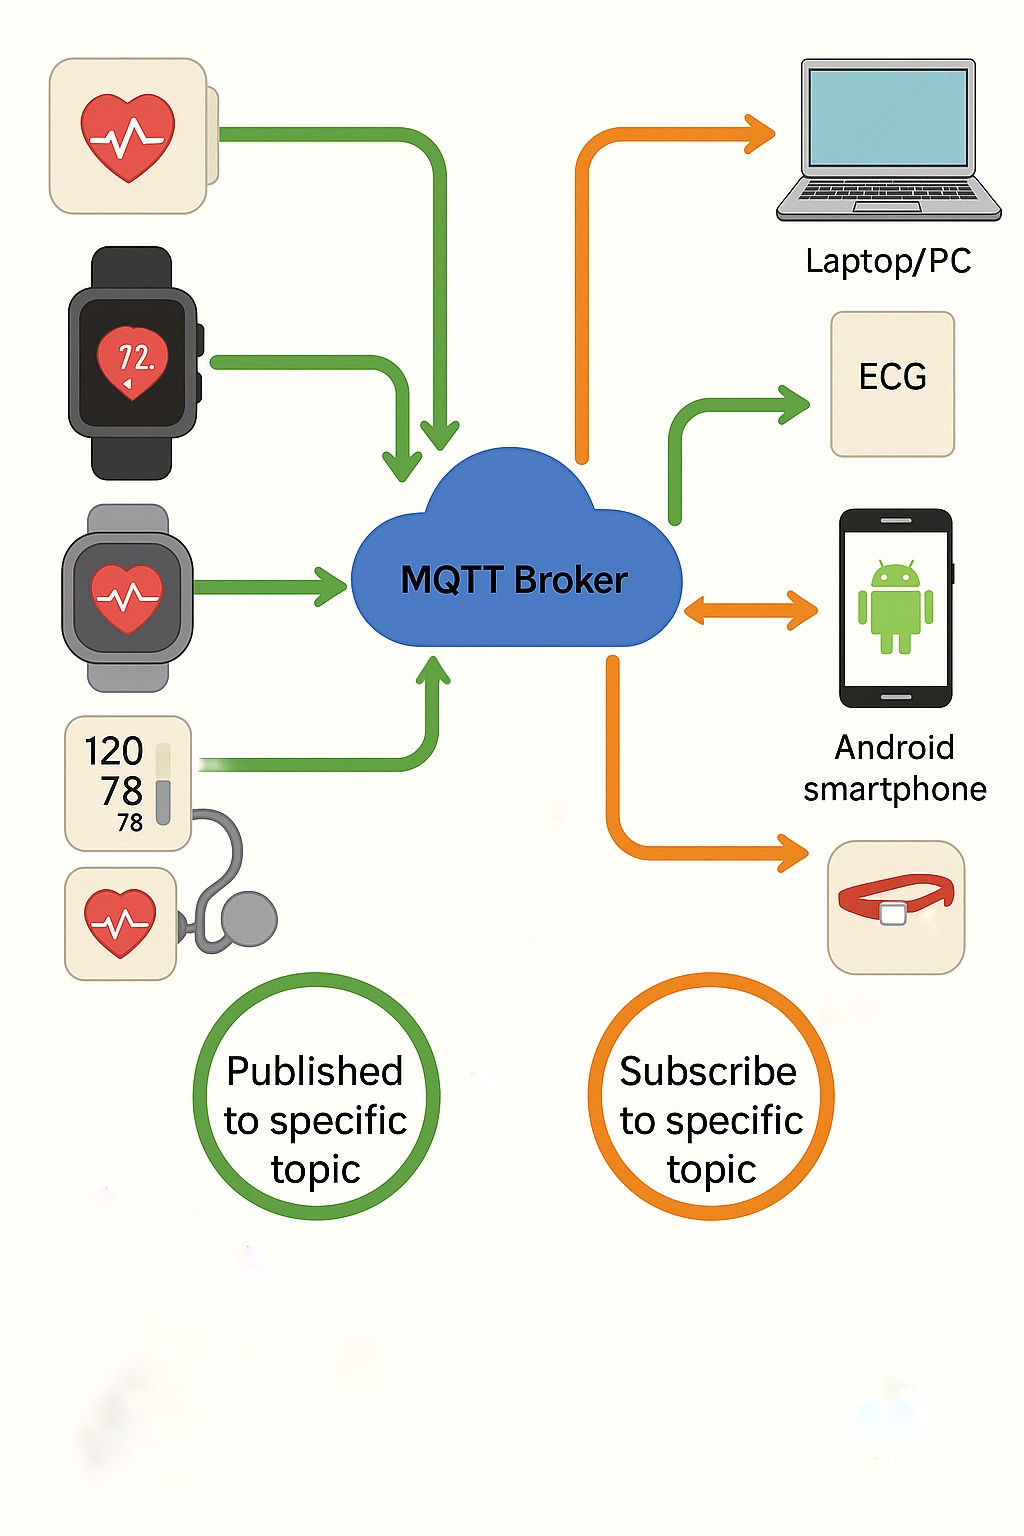
\includegraphics[width=0.4\textwidth]{img/MQTT_IoMT.jpg}
    \caption{Protocol MQTT en un entorn IoMT. Imatge extreta de \cite{mqttfig} i adaptada amb intel·ligència artificial.}
  \end{figure}

  \section{Altres protocols en l'entorn IoMT}
  Pel que fa a altres protocols, tot i que MQTT és el protocol principal emprat en aquest treball, també es considera l’ús del protocol Constrained Application Protocol (CoAP) com a alternativa o complement en la generació de trànsit. CoAP és un protocol pensat específicament per a dispositius amb recursos limitats en xarxes IoT. Funciona sobre UDP, cosa que li proporciona una latència molt baixa i un comportament lleuger, tot i que això també comporta certes limitacions pel que fa a la fiabilitat de la transmissió. 

  CoAP segueix un model client-servidor similar a HTTP però optimitzat per a entorns embeguts. Utilitza mètodes com GET, POST, PUT i DELETE, i permet observar recursos mitjançant un sistema d’actualitzacions automàtiques (observe). A diferència de MQTT, que és orientat a un model (publish/subscribe), CoAP és més adequat per a interaccions puntuals o consulta de recursos puntuals. En aquest treball, l’ús de CoAP es contempla per generar variabilitat en els escenaris de comunicació i per comparar comportaments de trànsit entre protocols amb estructures diferents. Això pot enriquir el dataset resultant i millorar la capacitat de generalització del sistema d’IA per a la detecció d’intrusions. 

  En l’entorn mèdic, també són utilitzats altres protocols d’aplicació com HTTP/HTTPS o bé Extensible Messaging and Presence Protocol (XMPP) Pel que fa a protocols de capa física, també es fa servir Bluetooth Low Energy (BLE), Near Filed Communication (NFC) o bé dades cel·lulars com NB-IoT que no seran usats en aquest treball.